%----------------------------------------------------------------------------------------
%	PACKAGES AND OTHER DOCUMENT CONFIGURATIONS
%----------------------------------------------------------------------------------------
% !TeX TS-program = pdflatexmk

\documentclass[a4paper,11pt]{scrreprt}
\usepackage[hscale=0.69,vscale=0.79,heightrounded,includehead]{geometry}
%\pagestyle{headings}
\usepackage{fancyvrb}
\usepackage[usenames,dvipsnames]{xcolor}
\usepackage{soul}
\usepackage{wrapfig}
\usepackage[english]{babel}
\usepackage{graphicx}
\graphicspath{ {../graphics/} }
\usepackage{floatrow}
\usepackage{babel}
\usepackage{csquotes}
\usepackage{caption}
\usepackage[labelformat=simple]{subcaption}
\usepackage[T1]{fontenc}
\usepackage{float}
\usepackage[backend=biber]{biblatex}
\addbibresource{references.bib}
\usepackage{epstopdf}
\usepackage{hyperref}
\usepackage{listings}
\usepackage{color}
\newcommand{\HRule}{\rule{\linewidth}{0.5mm}}
\definecolor{dkgreen}{rgb}{0,0.6,0}
\definecolor{gray}{rgb}{0.5,0.5,0.5}
\definecolor{mauve}{rgb}{0.58,0,0.82}
\usepackage{amssymb,amsmath}
\usepackage{abstract}

\addtokomafont{chapterprefix}{\raggedleft}
\renewcommand*{\chapterformat}{%
\mbox{\chapappifchapterprefix{\nobreakspace}%
\scalebox{5}{\color{gray}\thechapter\autodot}\enskip}%
}


%----------------------------------------------------------------------------------------
%	BEGIN & TABLE OF CONTENTS
%----------------------------------------------------------------------------------------
\begin{document}

\title{Realtime Classification Engine}
\subtitle{Msc Intelligent Systems Dissertation}
\author{Andrew Haines\\
	University of Sussex\\
	\texttt{ajh21@sussex.ac.uk}}

\date{\today}
\maketitle

\begin{abstract}
With the invent of processing platforms that allow for cheap, commodity hardware to run horizontally distributed applications at unprecedented scale, never before have we seen such an explosion of data collection and processing. Because of this abundance of processing power and ever cheaper storage costs, there is a growing trend to capture and collect events, limited only by what can be instrumented and regardless of an immediate requirement. These persisted events sit dormant in data centers waiting for their vast coffers to be harvested for valuable insights and application. Many of the algorithms and developments that have arisen out of this have relied on the fact that even though such sporadically collected data is noisy, with enough of it, the law of large numbers suggests that signals can still emerge and be fed into a new breed of intelligent systems\cite{bigdata}. The problem with this approach is that, although tractable to large institutions and organizations, smaller, more modest individuals will not have the infrastructure or financing to support such data collection even though their reach is enough to warrant its need. Tech startups in particular face this problem with a careful balancing of the business insights and user requirements they can provide at a trade off of vast equity deals in seeding rounds.\\

In this project we attempt to design and build a closed domain application that runs at 'big data' scale but on a single machine instance. The closed domain of the application is one of a classifier that, given an entity or event expressed in a feature space, it recommends suggested classes based on a continuous stream of online data input. The ideas and concepts that semantically define this recommender are nothing new but its implementation and structure is novel, excelling previous standards by making extensive use of modern computer architecture to process events far quicker than traditional techniques.

\end{abstract}

\tableofcontents

\chapter{Introduction}
More and more large institutions these days rely on the analysis of vast quantities of data to inform business decisions and provide performance feedback. From tracking the performance of advertising campaigns, constructing weather models, and powering recommendation engines, Big Data processing is rapidly becoming the cornerstone of the online technology industry. Large companies such as Google and IBM spend hundreds of millions of pounds in capex to construct and maintain the processing platforms required to mine this data. These systems are typically generic constructions developed across many thousands of machines and delivered company-wide to cater for all business units in the organization. Resources such as storage and compute time are then shared across all applications of the company. To accommodate this, either fully distributed but virtualised operating systems that coordinate a 'grid' of machines and networking topologies or complex multi processing core workhouse instances are used to execute such data hungry applications. There are many different paradigms and approaches for powering these systems but they all share one common drawback - these infrastructures come at the cost of an astronomical financial footprint, costing several hundreds of thousands of dollars for comparatively modest setups to multi million dollar investment for corporate scale facilities.

The focus of this project is whether the existing designs and ideologies of these approaches can be borrowed, blended and re-devised to create a system with a real life intelligent application that runs at big data scale but with a fraction of the monetary expenditure. If such a system is possible, the value to individuals where existing big data solutions are out of reach could be unprescended.

\chapter{Background}
\section{Big Data Processing Paradigms}
The current state of the art in these approaches fall primarily into three distinct camps.
\subsection{Batch Processing}
The first archetypical model for such computation is one that follows a batch processing methodology. The concept is that data is persisted onto a distributed file system in near raw form. Processing then operates on the data either as a one off task for insight analysis or bootstrapping purposes or, at periodic intervals that produce transformed data that can be used in downstream processes. To illustrate this, consider a possible implementation of a 'trending now' feature on a large web property's home page - used to inform users of what is currently popular on the domain at that time. \\

To determine this, the web property instruments all interactions with various content on its systems. This could be tweets sent from a mobile device app or news articles clicked on via a user's web browser - all events are logged to a central analytics system with a pre defined payload. This payload could contain information about the user\footnote{gender, age, personal preferences, etc}, the local time the event occurred at, information about the device, the content UUID interacted with... the tuple of data that could be chosen is endless. The analytics servers then typically place the event, via a messaging system onto the distributed file system\footnote{This file system is distributed in the sense that the data actually sits on multiple machines possibly in geo graphically diverse data centers but appear as if it is one contiguous structure of files.} in a '\texttt{rawevents-YYYYMMDDHH-xxxx}' series of files. A scheduled task then runs at say every hour and consumes these latest files, extracts named entities from them and contructs a histogram of their occurrences. The named entities are then ranked according to the histogram's frequency and the top x results are persisted into a '\texttt{trending-now-YYYYMMDDHH}' timestamped file. This comparatively tiny file is then sent to all the client facing webservers and powers the last hour's 'trending now' list.\\

Using the batch approach enables the data to be processed 'offline' in the sense that data is processed some time after the events have occurred.  This has a number of advantages over the cost of not being real time. Firstly, the programming concepts can be far easy to implement. Consider the calculation of a median value of a vast list of numerical objects. Using batch you would simply sort the list and pick the middle one as you have all the data for that given hour available. Indeed, if you choose to not remove the intermediate '\texttt{'rawevents'} files then larger periods can be scaled up by simply increased the file ranges. Handling in the event of error is also far easier as processing can easily be rerun. The other downside is that the demand on storage capacity is huge but, given the growing trend to capture all data and archive it for later insights, this tends to already be available.\\

There are 2 main concepts within batch processing that allow it to structure the control flow of the application.

\subsubsection{Map Reduce}
This technique is an adaptation of an old functional programming paradigm where by two phases of computation are established - the map phase and the reduce phase. Google took this paradigm and ported it to a distributed setting in 2004\cite{mapreduce}. The general idea is that during the map task, execution is moved to where the data is rather then data being moved to whether the executable code lies. The reason in the big data setting should be obvious as the IO costs involved in transporting vast quantities of data to executor machines is fair costlier and time consuming then moving a small executable to each of the machine that store the event files. Such machines are referred to as data nodes. Execution in the map phase then runs on the data nodes and is used to filter, transform and assign special keys to each record that this data node holds. The output, being typically alot smaller, 'shuffled' to reducer nodes which may (some IO costs) or may not (no costs incurred) be on different machines before finally being sorted by the special keys assigned during mapping. This allows all items assigned to a particular key to be available on a single reducer. In the case of the trending now example, this would equate to each instance of a named entity being sent to a single reducer so that it's component of the histogram - its particular count - can be computed (see Figure \ref{fig:MapReduceEx}). In 2011 Yahoo open sourced the HadoopMR\autocite{hadoopMR} module that forms part of the hadoop operating system.\\

\begin{figure}[h]
\centering
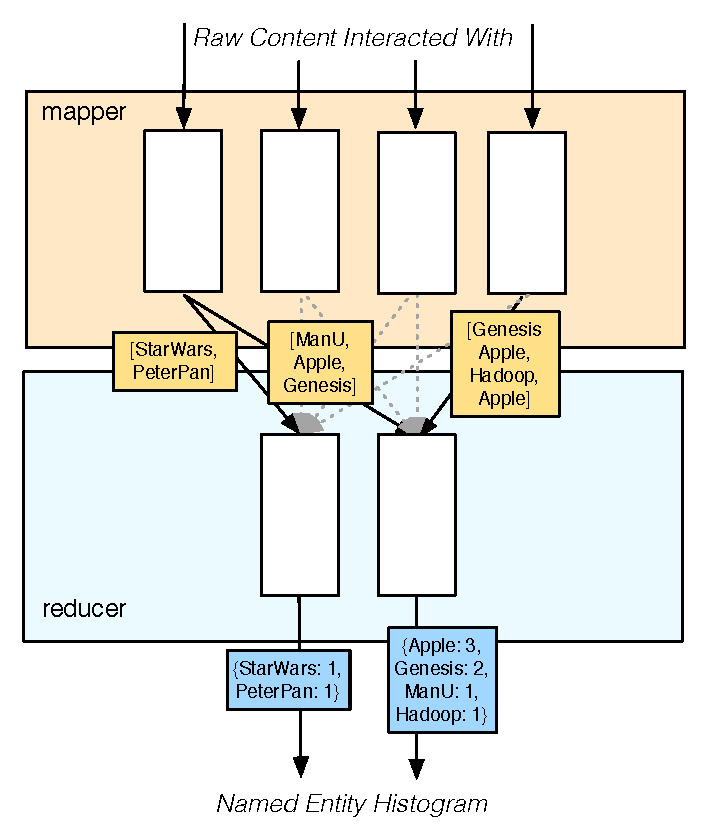
\includegraphics[scale=0.7] {MapReduceEx.pdf}
\caption{MapReduce Trending Now Example. For Brevity only 2 mappers are shown. The inputs to the process are the raw content data and the mappers determine which named entities are present. These are then keyed on the textual representation of the entity and all entities of the same name are sent to a single reducer. The output is then a frequency count of all named entities}
\label{fig:MapReduceEx}
\end{figure}

The problem with this approach is that, although it scales well when the distribution of the keys is uniform, in the face of skew in the key set, this bias is propaged down to the reducer load and can mean that a small number of machines can do the majority of the work. Also, as we have seen from the trending now example, the calculation of the distribution of terms is only one part of the entire process. It was assumed here that the entities of all the content that was interacted with had been previously computed. To do this using Map Reduce we would need another set of MR tasks that would extract the content from the raw events, normally only defined by the UUID, prior to the task described. The output is also just the raw counts, we would need a further step to then sort the entities by their counts and only persist the top x. This illustrates what typically happens with complicated MR applications in that a number of sub tasks of mapping and reducing have to occur with intermediate temporary files coordinating the data flow between them. This can be both limiting in how a application is structured and also inefficient due to unnecessary persistence of these temporary files. To solve this the DAG approach was devised:

\subsubsection{DAG}

\begin{figure}[H]
\centering
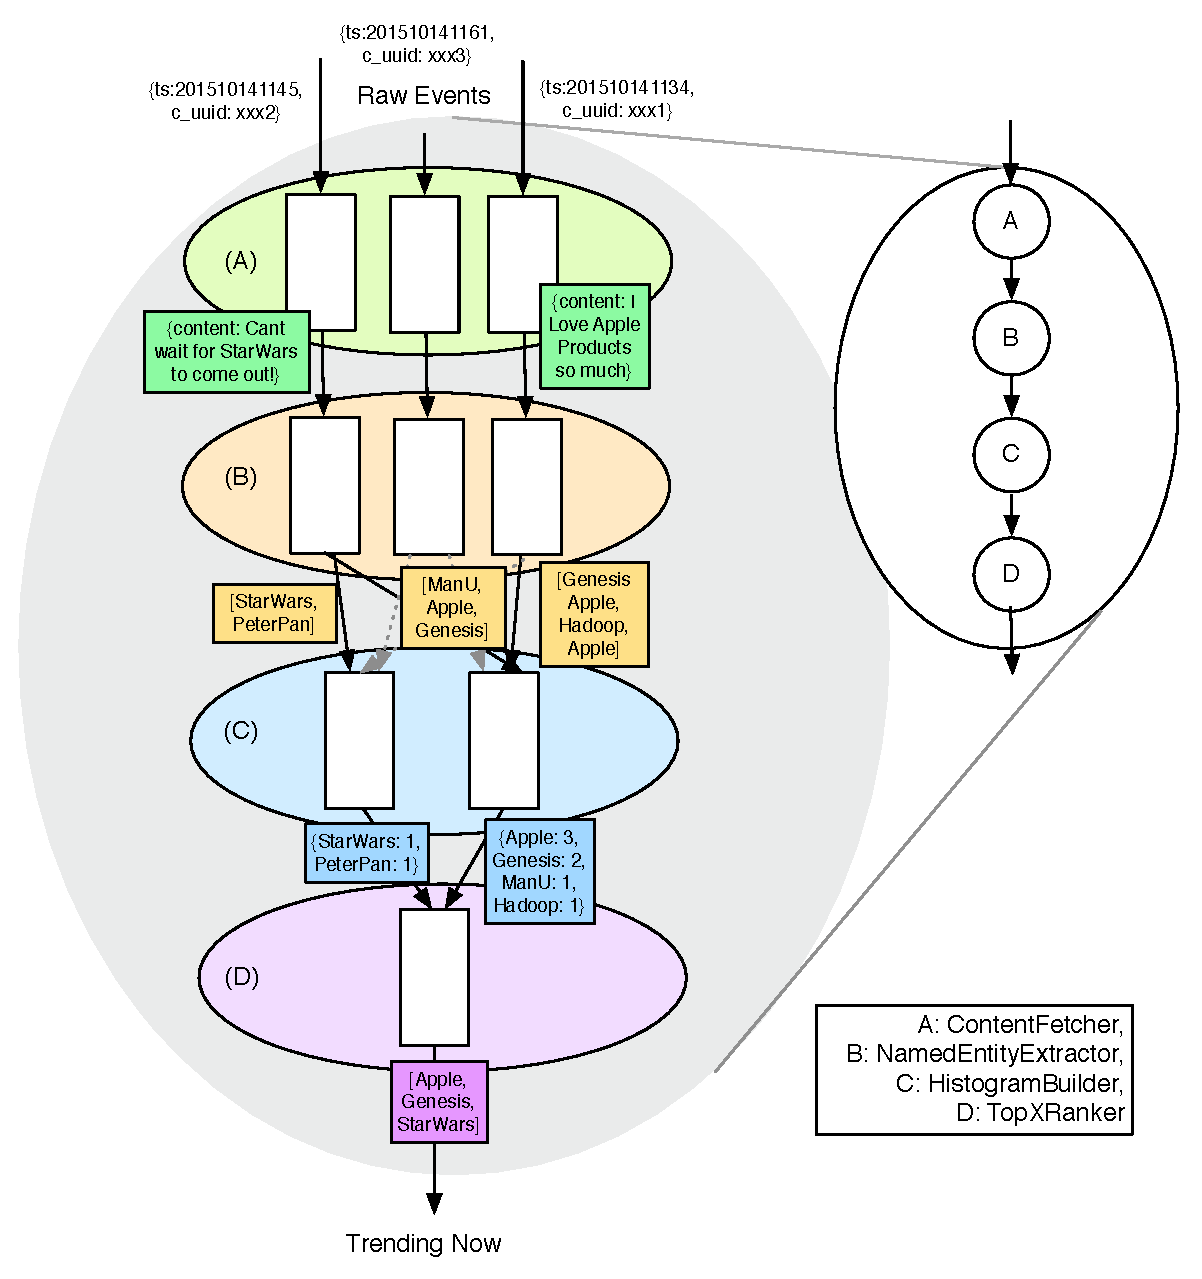
\includegraphics[scale=0.65] {DAG.pdf}
\caption{DAG Trending Now Example. In this example the entire application is shown, not just the histogram building. Data flows through the graph along the edges to the nodes. In this example, the DAG framework is able to determine that both the content fetcher and the name entity extractor need never move any data around and so the computation actually happens on the same nodes without ever having to write to disk}
\label{fig:DAGEx}
\end{figure}

The Directed Acyclic Graph\cite{dryad, spark-paper} approach tackles the deficiencies of MR by defining a graph of tasks that have to be executed concurrently. Nodes in the graph are sub tasks that need to be performed and the edges are data flows between them. Nodes are distributed as in MR by moving them to where the data is but there exists far more flexibility in how an execution flow can be maintained and structured. In the trending now example, a node can exist for extracting the entities of the file, where the determined entities are then fed into the distribution calculation node to obtain counts prior to another node that then filters out the x largest entities (see Figure \ref{fig:DAGEx}). Libraries such as tez\cite{tez-site} and spark\cite{spark-site} are two popular frameworks currently gaining traction in the industry.

\subsection{Stream processing}
One of the big problems with batch processing is that it is not real time. For most applications this isn't too much of a draw back but imagine budget caps on an advertiser spend. Waiting for the next hour's processing window to cut off an advertisers supply could be extremely costly. Assuming that processing never overruns\footnote{There is overhead with starting up distributed tasks that can easily make stall resource allocation and cause SLA's to be missed}, near realtime updates could be possible by reducing the processing window of the batch to a few minutes to help mitigate this issue but this isn't going to help a nuclear cooling processor from reacting to a sudden over heating. Stream processing provides a solution to this by processing events in a stream manner as they enter the system and distributed across a cluster of nodes. This means that events are processed, for the most part, either directly from the network bus or in a temporarily buffer, but never needing to be saved on the distributed file system. Processing is structured as a topology using concepts such as spouts and bolts to represent the data flow and processing respectively. In the trending now example, processing occurs in a very similar manner to that of the DAG approach. The difference being of course that at no point does a node get to see anything other than the current event. This is fine in our trending now example until we get to the ranking stage. \\

Choices have to be made in streaming about concepts like where an accumulating histogram is stored and for how long does it persist for? There is no point in keeping the histogram for all time as this defeats the purpose of the trending \textbf{\textit{\underline{now}}}. One option would be to reset every hour, assuming the behavior of the batch processing methodology - except that it wouldn't. A few seconds after the reset and there may not be enough data seen in the histogram to make accurate predictions meaning that periods just after each reset are inherently noise as the law of large numbers does not hold. Another approach would be a rolling window but this means that you need to keep all events in memory for each window. The larger the window the more likely to exhaust memory whilst smaller windows may not capture enough data. Also consider the median calculation mentioned previously. Without access to all the events, online versions such as a TDigest\cite{tdigest} need to be used which are far harder to implement and understand. Not only is stream based programming a lot harder but they are also extremely sensitive to the throughput coming and what can actually be processed. If your cluster is not large enough to process the influx of events coming into the system, then events are either dropped or buffered, reducing it's real time nature.\\

Obviously the upside of the stream approach, other than it's realtime operating behavior, is that it's also super fast as IO is reduced to bare minimum. Apache Storm\cite{storm-site}\footnote{a commonly used distributed stream processing framework open sourced from Twitter\cite{storm-twitter}. Apache Spark also offers a streaming mode but underneath the hood this is really a micro batch mode to approximate real time\cite{spark-streaming-paper}} claims to be able to process 1M events a second using just a 10 node cluster\footnote{It is worth mentioning that the author's experience of such throughput requires slightly more nodes in a real setting}. Furthermore, if storage capacity is deemed a premium, then this approach can allow big data processing to function without the need of a distributed file system. 

\subsection{High Throughput Systems}
On the other side of the technology spectrum, high throughput processing used in real time exchanges such as those within financial and scientific industries, are able to process huge streams of data but instead of scaling horizontally by adding more machines into a cluster, a single workhouse instance is used with multiple CPUs, huge memory addresses and dedicated transport buses that coordinate the data between. These are concurrent systems that are considered to scale vertically because obtaining more processing power and memory involves the reconfiguration of the instance itself by adding better CPU's or memory modules. These bespoke systems execute code that is specifically tailored to the underlying hardware which makes them incredibly efficient and able to outperform similar speced Hadoop or Storm clusters. Although typically favoring CPU bound tasks, these so called 'supercomputers' can still process vast amounts of data.
\begin{figure}[h!]

\centering
\caption{An example of a 2 core event driven data flow using disruptors to coordinate the transfer of events}
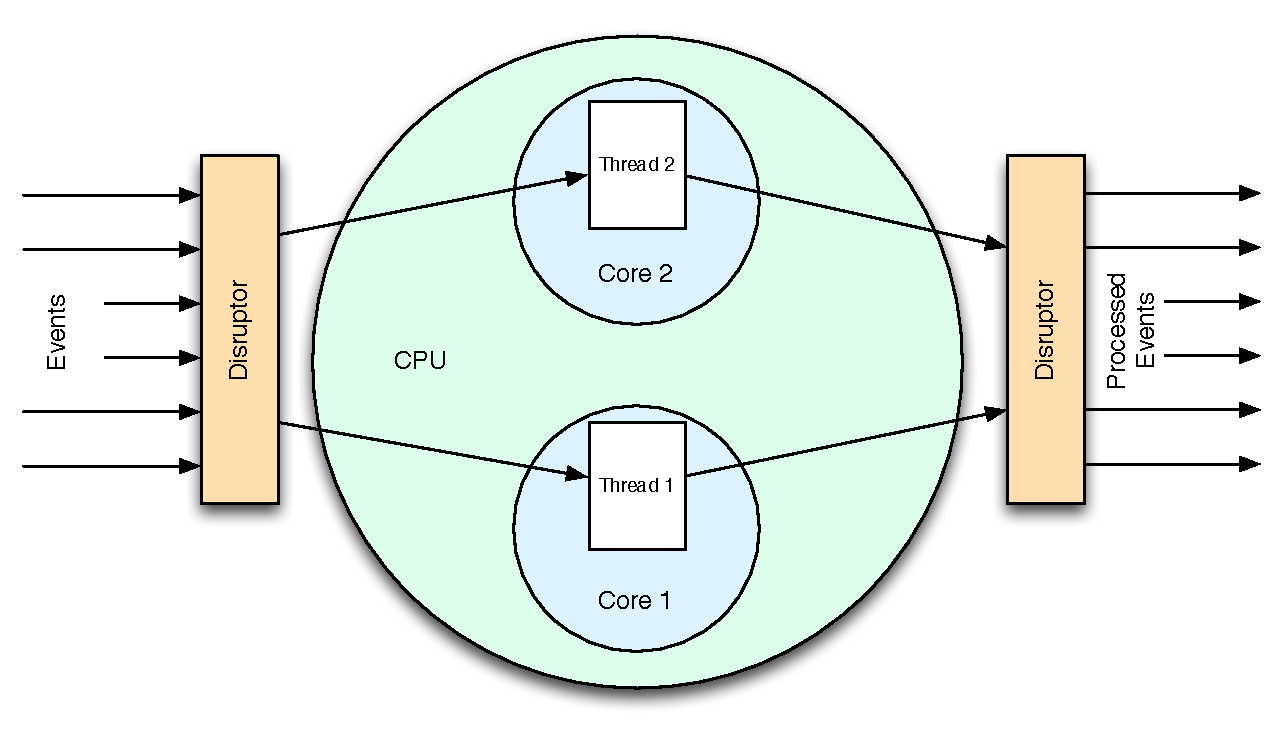
\includegraphics[scale=0.65] {disruptor-ex.pdf}
\label{fig:disruptor-ex}
\end{figure}

Further to this, the LMAX exchange in 2011 released a high throughput processing toolkit that borrowed from similar principles of software and hardware cooperation. Using techniques borrowed from synergising hardware and software, this toolkit is capable of supporting 25M events a second on a single commodity instance\cite{disruptor-paper}. This is not actual computational work mind, just moving events from one conceptual area of a program to another under concurrently safe conditions. None-the-less, achieving such high rates of transfer in in a thread safe manner is still highly impressive. It accomplishes this by using lock-less queues known as \textit{disruptors} that exploit a perfect \textit{mechanical sympathy} between high level programming paradigms and the under lying hardware infrastructure. The basic idea is that disruptors can act as brokers for events, passing them to different areas of code that may or may not be on different threads. This enables event driven design where threads are only used to pin execution to a particular CPU core\cite{processor-affinity}. These long running threads then can operate on the events from the disruptor using the single writer paradigm which ensures that write contention is no longer a concern and only care about visibility to other reader threads need be considered(see \ref{fig:disruptor-ex}). The worker threads can then pass events through the system without costly synchronisation and thread context switching.

Disruptors obtain their ultra fast design by utilising cache line structures and memory barriers present on modern cpus. They are essentially queues implemented in ring buffers where the majority of access is completely unsynchronised - care only be taken to ensure that threads have visibility of events on the buffer. Using a volatile pointer to the index of the buffer, as long as all event processors do not read past the writer position, no locking is required. 
\floatsetup[figure]{capposition=beside,capbesideposition={top,right}}
\begin{figure}[h]
\centering
\caption{The ring buffer at the heart of the disruptor design. For clarity the writer and reader positions are illustrated as if they are concerns of the Producer and EventProcessor respectively - however this is not the case in implementation as the ring buffer owns the pointers in order to ensure \(writerPos < readerPos\)}
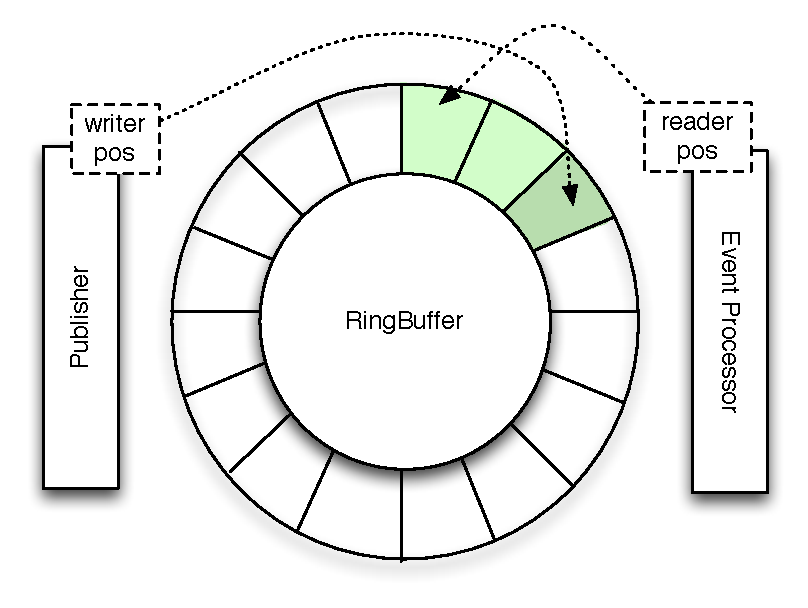
\includegraphics[scale=0.65, trim=0 10 0 0, clip=true] {ringbuffer.pdf}
\label{fig:ringbuffer}
\end{figure}

In the one scenario where the reader and writer are pointing to the same index, CAS operations are used to \textit{busy wait} on mutual exclusivity on this pointer but without coordination amoungst many threads. Under low contention, CAS operations are extremely efficient. Furthermore, as long as the invariant of \(writerPos > readPos\) is held, unlike other cyclic buffers, no end pointer is needed as data can be overwritten when the buffer wraps around.

\section{Machine Learning Applications at scale}
One of the major fields to utilise such large quantities of data is Machine Learning. Tasked with finding systematic patterns in the data and providing classifications and recommendations, ML techniques are used throughout large tech companies to enrich the user experience and provide business analytics. So much so that further abstractions have been provided on top of the data processing paradigms already discussed to enable quick implementations of standardised algorithms and techniques. Libraries such as Mahout\cite{mahout-site} run on top of the hadoop platform and provide scalable interfaces to Logistic Regressors, Random Forests, Collaborative Filtering, etc that engineers can use out of the box at scale. All they need do is chose an algorithm, direct it to the data they wish to be analysed with appropriate hyper parameters and the framework does the rest. Spark in fact is so popular with machine learners that it has bundled its MLlib library as part of the core kernel of the framework, focusing on ML at it's heart. When we move into the streaming implementations as provided by Spark's MLlib library for example, the same considerations mentioned earlier need to be applied in the development of how data is structured and processed at each stage of the computation.\\

Similarly, the popular scientific computing package MatLab offers parallel computing support via its Distributed Computing Toolbox that can utilise 64 CPU cores and beyond, exposing ML libraries to vertically scaled options.

\chapter{Motivation \& Scope}
As seen, there exists a plethora of frameworks and libraries that enable large machine learning applications to be developed at unprecedented scale. But these approaches all have their draw backs. With typical server instances costing upward of \$5K, even a modest Hadoop setup can cost in the order of \$50K. Any serious implementation also needs to consider fault tolerant deployments typically with hot-hot mirrored replications in geographically disparate locations. Assuming that data center and rack space need to be acquired, once on going maintenance costs are also factored in, costs to build such an infrastructure can easily approach the \$500K mark. This investment is likely to be way out of reach for startups and other small institutions without serious seeding.

To combat these extreme up front infrastructure costs, services such as Amazon's EC2 and Google's ComputeEngine enable clients to 'rent' capacity from their own internal cloud infrastructures. Instances can be acquired on an 'as-needed' basis where entire Hadoop or Storm topologies can be spun up in minutes. This proves extremely cost effective for the periodic applications\footnote{say a TV broadcast or sporting event requiring data capture} but for more long term applications, although the up front costs are lowers, long term costs can easily dwarf investing in dedicated hardware\footnote{Whilst working on EA's SimsSocial online game supported by a 200 node cluster, its yearly EC2 bill came to \$1.1M}. It could be said however that if such vast resources are required then presumably there is a business model in place to support it. The downside is that moving off such a platform is extremely difficult as migrating data and code from a cloud system without down time is a monumental effort.\

Cloud services are also not appropriate for certain types of applications. As they are typically virtualised, performance of a single instance is also dependent on other users congesting the resources surrounding it. CPU's, main memory contention, rack IO and network switching can all add unwanted variance to perceived performance making guaranteed response times difficult to predict. For real time applications to work properly, the stream of data in and out need to ideally operate at a consistent rate.\\

When considering bespoke, vertically scaled instances, cost is also the main inhabiting factor. A modest Cray XC30-AC retails at around the \$500M mark which again puts it out of the reach of all but the largest organizations. The difference between the two approaches however is that Hadoop is a platform for running on commodity mass produced hardware that can be scaled outwards as and when extra capacity is required. Once the XC30-AC is exhausted of capacity, expanding the system is a hugely expensive task. Furthermore, these sorts of systems require bespoke knowledge of the underlying hardware. Specialised engineers qualified to operate such machines further compound the expense of such operation. 

Dealing with such data is clearly a monumental effort and, as such, a reflective degree of supporting assets is clearly going to be required. As we have seen, one of the big advantages of distributed operating systems such as Hadoop and Spark is that they act in a very open domain - that is to say that they can solve a theoretically unbounded scope of problems. The ML libraries we discussed operate on these open domains and provide abstractions for a specific type of application - essentially restricting the domain. These layers of abstractions, although convenient from a development and resource sharing perspective, coming at the cost of performance. As the applications that sit on top of the open domained platform are unknown, mechanical symphony is not possible even though the type of applications that use the machine learning libraries are constrained. Consequently, efficiencies are rife in the world of the distributed platforms where the tradeoff between simplicity, performance and cost has been focused on the former at the expense of the others\footnote{There is an argument that, in large institutions, the cost of engineers and bug maintenance where the focus is on simplistic systems actually out ways the infrastructure costs.}\\

Today's modern off the self servers now come equipped with multiple cores. A 24 core Dell PowerEdge R730xd retails at around \$20k which should be considered a sensible, reasonable and comparably modest investment by most standards meaning that such high CPU specs are possible on a budget. By both constraining the problem domain and employing code that encourages a symbiotic harmony between components whilst capitalising on all available CPU cores of the underlying infrastructure of modern commodity hardware, the scope of this project is to build an intelligent real time system that runs at big data scale without the enormous investment costs required by the existing solutions available. 

To frame the task appropriately, the system is a real time classifier that, given a stream of labelled event data, builds a temporal model that reflects this input based on positioning in the events feature space. When an unseen and unlabelled event comes into the system, the event is provided with an intelligent label based on its internal model and the to-be-classified event's description in feature space. As the structure of the data changes, the model also reflects this change so that the classifications returned are representative of the current state of the environment. To provide an appropriate real world application for such a system, consider an adapted trending now feature like the one already discussed. This trending now provides a view into popularity of a site except with the additional ability to provide 'personalised' trends. To give an example, consider a user that has a previous history of interactions with say technology. When a new iPhone is released, such an entity might triumph over the new One Direction album that maybe popular for other types of users at that moment in time. In this setting, the events that enter the system are user interactions with content. These events are reflected as a tuple of data that can define them in a feature space such as age, location, previous category of interests, time of day, gender etc. The label is then the named entities extracted from the content that they clicked on. When classification occurs for a given user on what their top trends are, the system then returns the top n labels that they are most likely to be assigned to. Figure \ref{fig:featurespace} represents the setting in a spatial context.
\floatsetup[figure]{capposition=beside,capbesideposition={top,right}}
\begin{figure}[h]
\centering
\caption{Given a trival example of 2 predictors of age and geolocation, users can be positioned in a feature space to predict the entities they are interested in. In the case of the red user, a prediction can be made that it is similar to the named entities clicked on by the users around it.}
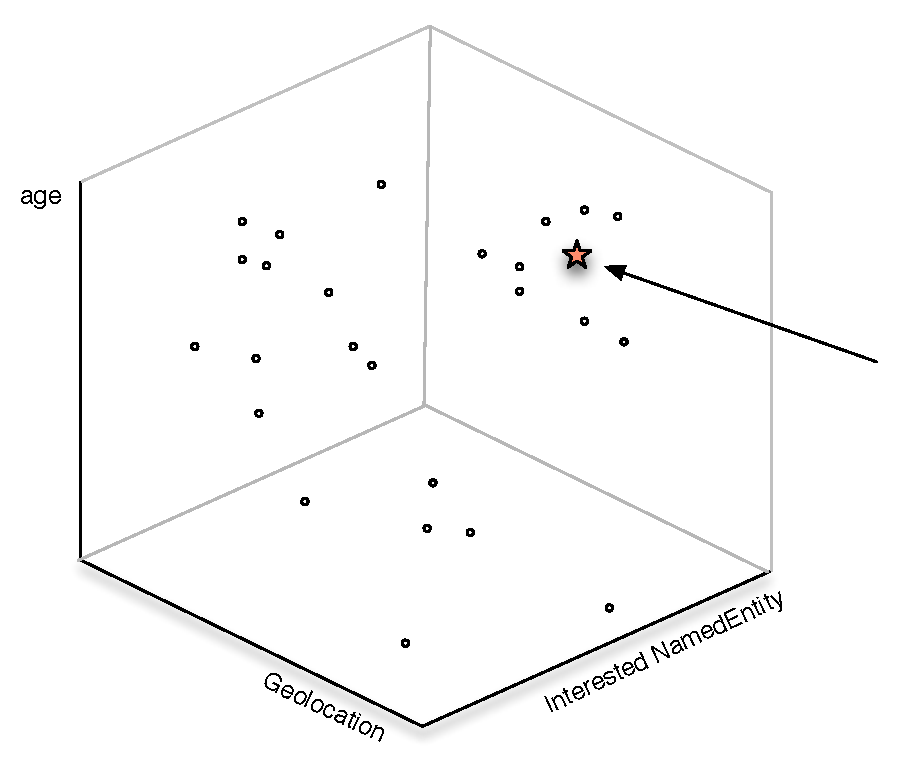
\includegraphics[scale=0.65, trim=0 10 0 0, clip=true] {featurespace.pdf}
\label{fig:featurespace}
\end{figure}

\chapter{Design}
\section{Overview}
The system proposed is one that places a synergy between the hardware and software at its heart, maximising not just all components of the underlying architecture but also ensuring that each component is utilised as efficiently as possible. The major components considered in this design:
\begin{itemize}
\item I/O bus
\item Main Memory
\item CPU cores
\item L3, L2, \& L1 cache lines
\end{itemize}
To understand how these components can be specialised, it is important to discuss how they work and what their role is in the overarching design of the system 
\subsection{Hardware components}
\subsubsection{I/O bus}
Like all internal system buses, the I/O bus is responsible for moving data from an auxiliary part of the computer to the CPU. I/O buses normally exclude main memory access and focus on components such as keyboard input, audio or, in the case interested in this project, network communication. Any data bound server instance like the one in question in this project requires extensive use of the networking interface, so much so that network is the primary bottleneck in such systems as IP packets are marshaled,copied and de-marshalled around the system using the I/O bus as its main \textit{highway} to all components. To ensure that this part of the system is as uncontended as possible, focus needs to be applied to reduce the overhead. In particular, the system keeps all marshalling and demarshalling as conservative as possible and uses the I/O bus to keep, as much as possible, this data away from main memory detours and interfaced directly with the CPU cores.
\subsubsection{CPU Cores}
In recent times we have seen Moores Law\footnote{A law describing the linear trend of core clock cycles/die-size over time} being upheld by the fact that, although clock speeds on single dies are plateauing due to physical constraints of heating and fixed atomic size, the number of clock cycles in a given CPU is still increasing due the addition of multiple cores on the same physical die. The Intel i7 CPU for example is fitted with up to 8 cores on a single die. Moreover, modern servers can be found with multiple CPU's means that upward of 24 cores can be found in modern systems.

Traditional procedural programming is still possible on such architecture but will be limited to a single core. Within a multitasking environment such a design is ok but when considering a single server instance responsible for a single task, threading or multi process design needs to be considered. A common technique is to use the threading model that conceptually isolates a unit of atomic work to occur concurrently with other threads. In a typical web server for example, the threading policy needs to be carefully tuned to obtain the maximum performance. Too few and the system is under utilised whilst too many results in contentious context switching. The problem with the threading model is it does not really reflect with is happening in the underlying hardware. Under the hood, processing is signaled using interrupts\footnote{In fact threading is achieved by \textit{multiplexing} these interrupts so that the illusion of atomic and concurrent units of work can be achieved} which tell the cpu which execution address to jump to next when IO events are received. The only real concurrent unit of work in a computer is what is actually executing on a CPU core at any one time. As such, the threading policy of this system should be such to mimic this behavior - 1 thread for each CPU\footnote{Ideally using thread affinity where the OS is instructed to only execute a given thread on a given core} with an event driven methodology to reflect the interrupt nature of the supporting buses.

\subsubsection{Main Memory and Caching}
\floatsetup[figure]{capposition=bottom}
\begin{figure}[h]
\centering
\caption{Illustration of the different cache visibilities based on a 2 CPU, 4 core setup}
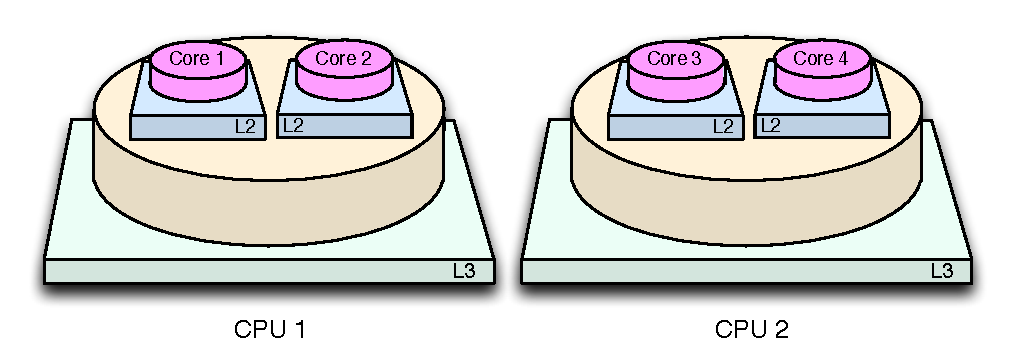
\includegraphics[scale=0.65] {cachelevels.pdf}
\label{fig:corecachedesign}
\end{figure}
Modern CPU's gain extensive performance improvements by using dedicated caching that sits on top of the processing units. These small but extremely fast memory elements sit directly within the CPU die allowing for frequently required data to be accessed at a fraction of the cost of accessing main memory. Caches map main memory in the form of cache lines that are contiguous areas that exploit both temporal (items used at time \(t\) are likely to be used at time \(t+1\)) and spatial locality (items located near each other are likely to be used at a similar time). Data of a cache line is moved from slow main memory into fast cache memory as it is being accessed. To optimise it's use of memory, the system needs to exploit the locality principles of the cache lines, avoiding cache misses and keeping data as close to the CPU for as long as possible. 

The downside with such design is that when data is sitting in cache lines, it is not guaranteed to be visible in other parts of the system. Data stored in the L2 cache of Core 1 of Figure \ref{fig:corecachedesign} cannot be seen in Core 2. Furthermore, data in the L3 cache of Core 3 cannot be seen by Core 2. Consequently, care has to be taken to set up correct memory barriers\footnote{In java for example, memory barriers are created using the \texttt{volatile} \& \texttt{sychronized} keywords and the \texttt{Sync} primatives from the concurrency package} when data is needed to be flushed back into main memory for other cores to see it.

\floatsetup[figure]{capposition=bottom,capbesideposition={top,right}}
\begin{figure}[h!]
\centering
\caption{Although there are multiple cache lines present in modern designs, as observed here the real speed benefit is avoiding main memory and as such this is the focus in this project.}
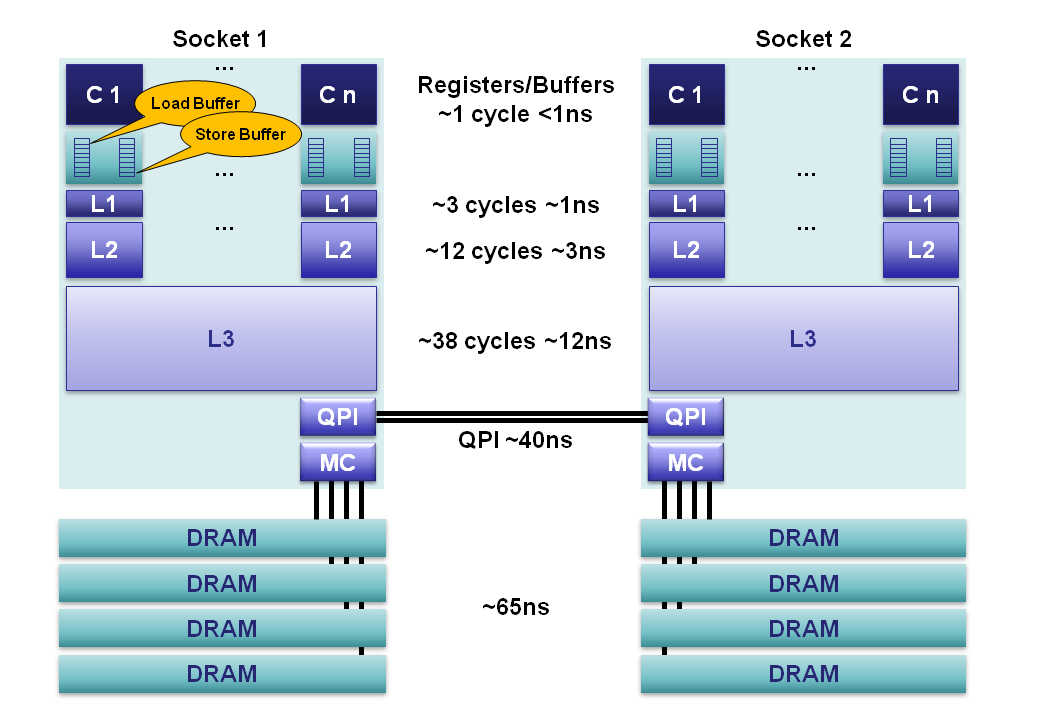
\includegraphics[scale=0.5] {cachelinespeed.png}
\label{fig:cachelinespeeds}
\end{figure}

\subsection{Software Architecture}
As previously mentioned, in order to optimize all the hardware components mentioned above an event driven design needs to be adopted, filing off to threading only to distribute the computational load across processing cores. Once events have been handed over to a specific core, the thread that owns the event also \textit{owns} its visibility completely. That is to say that no other thread is expected to have read or write access to it whilst in this core's care. This allows the application to enforce locality benefits in the data without worrying about visibility to other threads and thus providing a setting that minimises the copying of cache lines to and from main memory and satisfies the desire to keep data as close to the Core as possible. When the core is finished with the event, a model of releasing ownership of a collection of events at once is adopted by \textit{pushing} these events downstream to another component where visibility is required. 

To facilitate the movement of these events from the input stream into the care of dedicated cores and finally, back into main memory, the use of the disruptor queues already mentioned is selected. Note only are these queues lightening fast but they also put in place the required memory barriers mentioned to, like a runner in a relay, pass off ownership of the event once finished. A rough architecture plan of the system is presented in Figure \ref{fig:architectureoverview}

\floatsetup[figure]{capposition=bottom,capbesideposition={top,right}}
\begin{figure}[h!]
\centering
\caption{The main components and data flows of the system}
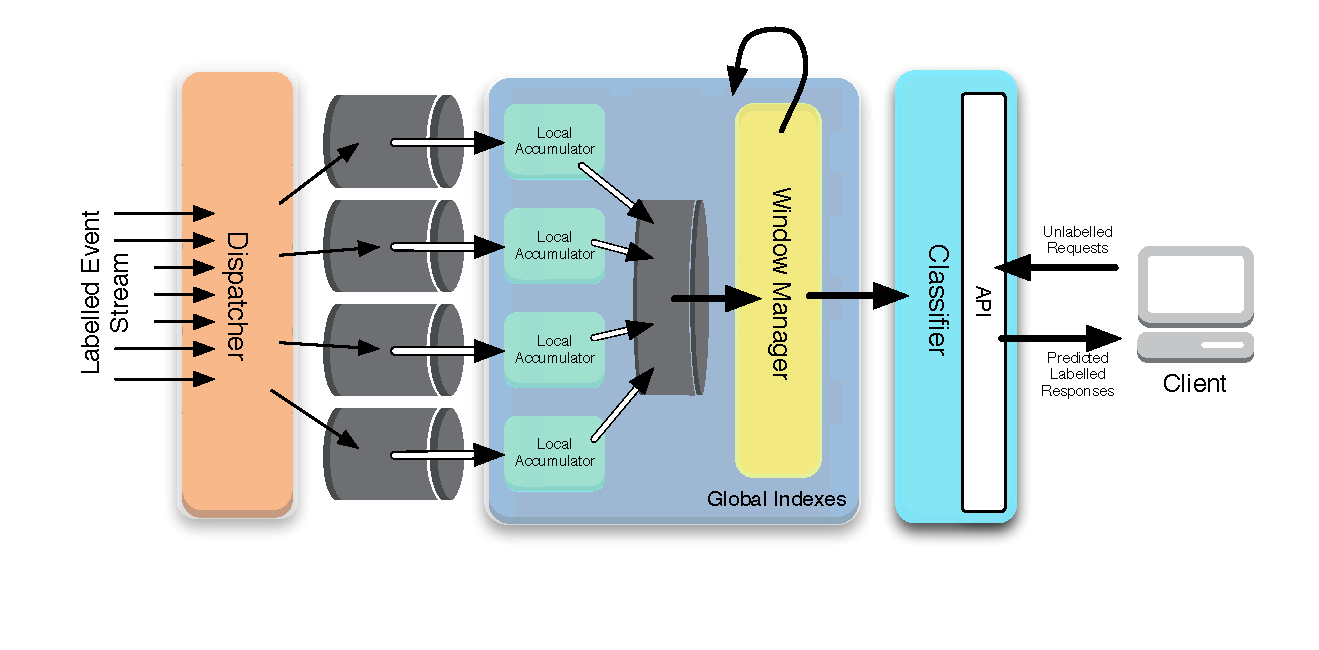
\includegraphics[scale=0.72, trim=35 50 0 13, clip=true] {architectureoverview.pdf}
\label{fig:architectureoverview}
\end{figure}

A rough overarching view of the system. Event driven philosophy. Completely lockless. Architecture diagram and rough description of the different components.
\subsection{Execution Modes}
\subsubsection{Async}
\subsubsection{Sync}
Discussion on the Asnyc and Sync modes of execution
\section{Naive Bayes}
Discussion on how naive bayes works and it's applicability for the task to achieve the classification given the above design.
\section{IO}
Some bit about how IO is the bottle neck in most systems
\subsection{Selectors}
Description on how selectors work and how they are a better fit model to threading as they mimic interrupts on the OS level.
\subsection{Protostuff}
Description of why protostuff was chosen (easy to define. quick etc). The off heap byte buffer implementation added as part of this project.
\section{WindowManager}
How the window manager maintains a rolling window view of accumulated representations of the event stream. Takes input from all the different accumulators based on the execution mode.
\section{Accumulators}
A description of how the accumulators can sit on the cache lines reducing copying into main memory. Talk about the ordering of the accumulators so that most frequently seen slots (prior and posterior combinations) so they fit in cache lines and dont need to be flushed to main memory
\subsection{Instances}
How the different instances interact with each other
\subsubsection{Local Instance}
local mode accumulators. 1 per cpu, supports writes and inherits from global
\subsubsection{Global Instance}
Provides a read only view of the window manager's view of all accumulated captured events. 
\subsection{Types}
How we assign meaning to each of the accumulator slots
\subsubsection{Discrete}
Simple a count of prior/posterior pairs for naive bayes - one for each slot. How they are accumulated together both on a per event level and on a per accumulator level
\subsubsection{Continuous}
multi slot length to capture parameters of distribution models. How they are accumulated together both on a per event level and on a per accumulator level
\chapter{Implementation}
Discussion on how the design is implemented. Only areas of implementation note are provided as this section could get out of hand! Core interfaces such as EventConsumer, Accumulator, FeatureHandler, ClassificationHandler etc.
\section{Maven Modules}
How the application is structured and the reasons why for extension and customisation
\section{Distributions}
How the distribution framework for continuous features is defined 
\section{Configuration}
overriding classpath configuration of jaxb objects.
\section{Testing}
How the DataSet classes abstract the test and training sets and produce their results.
\chapter{Performance}
\section{Classification Performance}
PerformanceTest results. AUC curves on the different data sets tested
\subsection{Synthetic Test}
Synthetic test to see if it can learn multivariate distributions in the presence of noise. Also mention how it is used in the load test to generate BigData equivalent volumes.
\subsection{Adult Wages}
A classification Task
\subsection{Space Shuttle}
A regression Task
\section{Throughput Performance}
LoadTest results. TCP vs UDP
\chapter{Conclusions}
\section{Results}
Discussion on how the results presented in the performance section compare with other systems.
\section{Limitations}
No FeatureExtraction.
\section{Future Work}
Plugging in more classifiers. Spatial models such as RBF's etc
Static analysis should be conducted,
Bucketed Continuous accumulator types

\printbibliography

\end{document}